\chapter{Exploratory Data Analysis}

In this chapter, we are looking only at the first innings of the games, and only those games in which the full 50 overs were played. The 
reason for this is the models we will build are going to try and predict a score as if a full innings has been played. \\

We begin our exploration of the data with a look at how the density of the runs scored per fall of wicket changes. This has been done for each
individual team in the dataset, and in figures \ref{ovrdens1fow}-\ref{ovrdens9fow}, we can see how this evolves.  

\begin{figure}[h]
    \centering
    \begin{minipage}{0.4\textwidth}
        \centering
        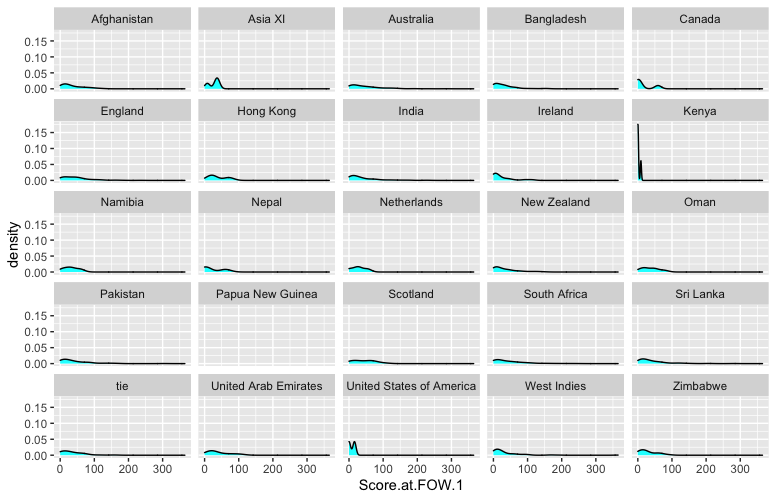
\includegraphics[scale=0.3]{figures/fow1density.png}
        \caption{Density of all teams for first wicket falling}
        \label{alldens1fow}
    \end{minipage}
    \begin{minipage}{0.4\textwidth}
        \centering
        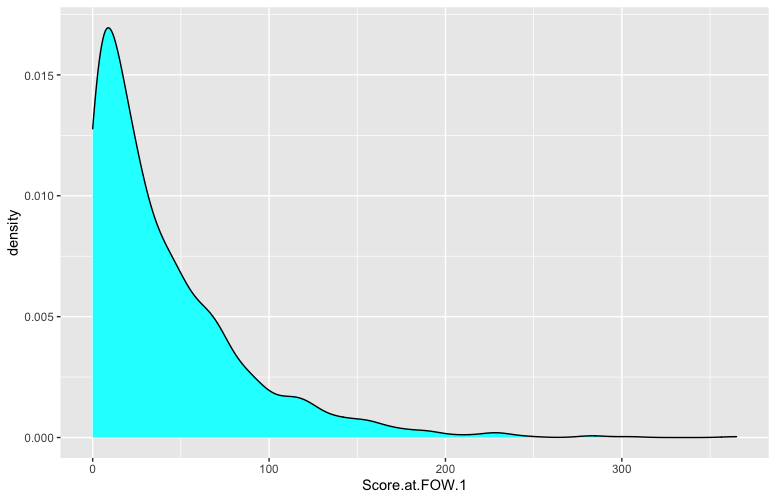
\includegraphics[scale=0.3]{figures/fow1densFull.png}
        \caption{Overall density plot for FOW 1}
        \label{ovrdens1fow}
    \end{minipage}
\end{figure}

\begin{figure}[h]
    \centering
    \begin{minipage}{0.4\textwidth}
        \centering
        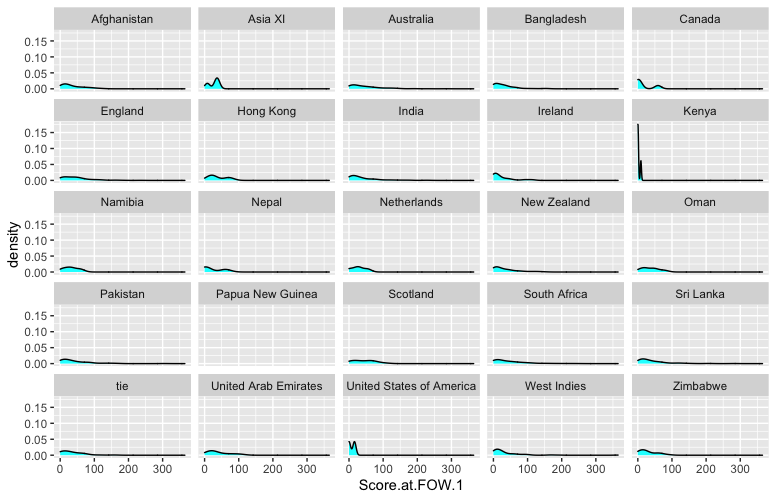
\includegraphics[scale=0.3]{figures/fow1density.png}
        \caption{Density of all teams for first wicket falling}
        \label{alldens5fow}
    \end{minipage}
    \begin{minipage}{0.4\textwidth}
        \centering
        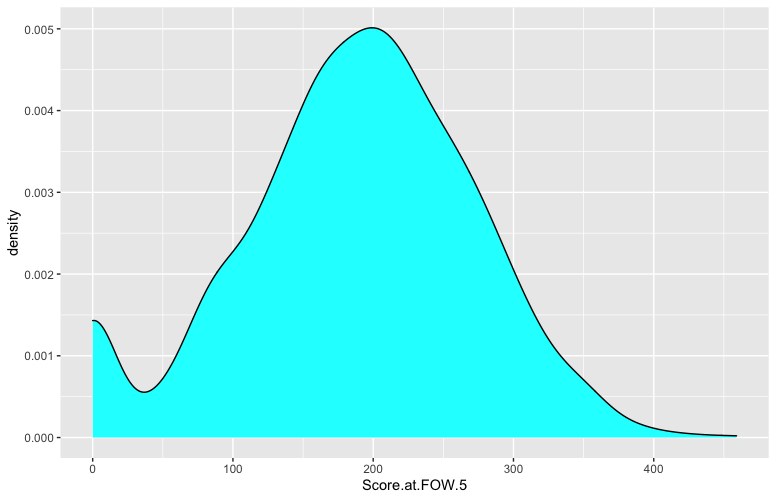
\includegraphics[scale=0.3]{figures/fow5densFull.png}
        \caption{Overall density plot for FOW 5}
        \label{ovrdens5fow}
    \end{minipage}
\end{figure}

\begin{figure}[h]
    \centering
    \begin{minipage}{0.4\textwidth}
        \centering
        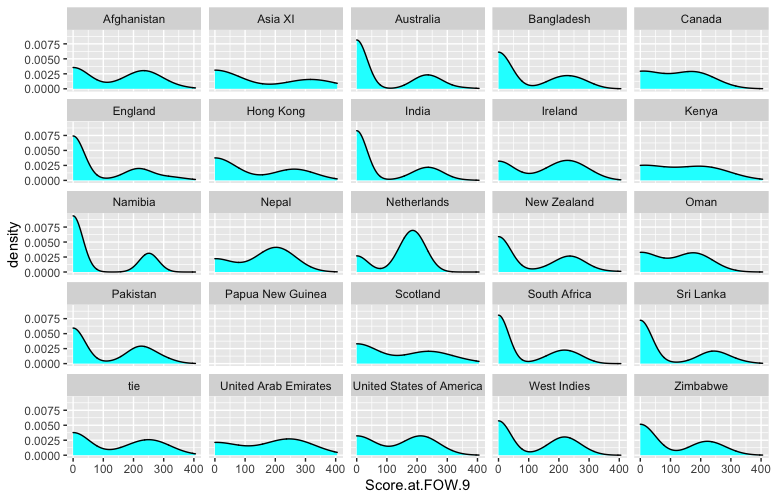
\includegraphics[scale=0.3]{figures/fow9density.png}
        \caption{Density of all teams for first wicket falling}
        \label{alldens9fow}
    \end{minipage}
    \begin{minipage}{0.4\textwidth}
        \centering
        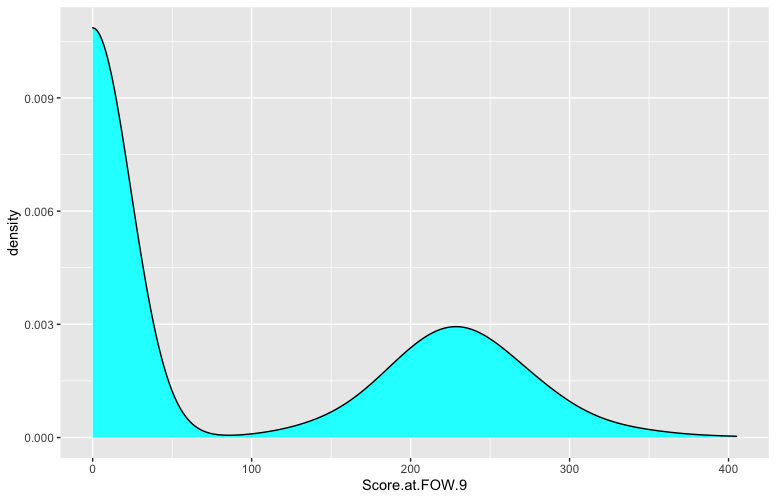
\includegraphics[scale=0.3]{figures/fow9densfull.png}
        \caption{Overall density plot for FOW 9}
        \label{ovrdens9fow}
    \end{minipage}
\end{figure}

In \ref{ovrdens1fow}, we see the density is heavily skewed to the left. This makes sense, as the bowling team will presumably be starting 
their innings by using their best bowlers, who will be hunting to get wickets early on. In \ref{ovrdens5fow}, we see a much more normally distributed
density function. But in actual fact, we see this interesting second, smaller peak appearing lower down in the score. Does this make sense? It's certainly 
not suprising. What these two peaks exemplify is the fact games can go heavily in favour of the bowling team, which can be seen in the first small peak,
wherein they have taken a lot of wickets in quick succession, meaning the later order batters are coming in earlier than usual. Secondly, it shows when the 
batting team is having a good day, because we have this much larger peak around the 200 runs mark.\\

Finally, in \ref{ovrdens9fow}, we can see that the earlier bowlingadvantage peak is much higer, because the lower order batters are traditionally less skilled 
at batting, and so the bowling team have a distinct advantage in taking wickets against these players. But we also see the second, batting-favoured peak is no much lower.
This corresponds to the scenario in which the earlier batters have laid a good foundation of the game, and the lower-order batters have not had to contribute much to the score.